\documentclass[]{article}
\usepackage[a4paper, total={7in, 10in}]{geometry}
\usepackage[OT4]{fontenc}
\usepackage[polish]{babel}
\usepackage[normalem]{ulem} % strikethrough
\usepackage{graphicx}
\usepackage{float}          % force figure by [H] argument
\usepackage{color}          %May be necessary if you want to color links
\usepackage[hidelinks]{hyperref}       % Clickable ToC
\hypersetup{
	colorlinks=false, %set true if you want colored links
	linktoc=all,     %set to all if you want both sections and subsections linked
	linkcolor=blue,  %choose some color if you want links to stand out
}

\newcommand{\SubItem}[1]{
	{\setlength\itemindent{15pt} \item[-] #1}
}



% metadata
\title{PERT diagram creator}
\author{Pawel Blaszczyk}
\date{Programowanie Aplikacji Webowych\\[0.5em]
	Projekt Zaliczeniowy\\[1em]
	2023/2024}

\begin{document}

\maketitle

\begin{abstract}
Dokument opisuje projekt aplikacj webowej przeznaczonej do tworzenia i pracy z diagramami PERT (Program Evaluation Review Technique), które używane są do planowania projektu i wyznaczania w nim ścieżki krytycznej.

W projekcie przedstawiono opis docelowej aplikacji (częściowo wykraczający poza projekt zaliczeniowy), wersję MVP (zakres projektu zaliczeniowego) oraz poszczególne elementy projektu, a w szczególności:
\begin{itemize}
	\item Plan projektu w postaci historyjek użytkownika
	\item Architektura oprogramowania (w tym diagramy klas i interacji)
	\item Opis wybranego stosu technologicznego
	\item Szczegóły implementacji
	\item Procedurę wdrożenia aplikacji na platformie Azure
\end{itemize}
\end{abstract}

\tableofcontents

\newpage

\section{Opis aplikacji}
Aplikacja ma za zadanie umożliwienie użytkownikowi zbudowania diagramu PERT (Program Evaluation Review Technique) na który składają się kamienie milowe (milestone'y) oraz zadania (task) pomiędzy nimi.

Użytkownik może umieszczać poszczególne kamienie milowe na obszarze roboczym oraz tworzyć połączenia między nimi. Połączenia symbolizują zadania do wykonania. Istnieją dwa specjalne kamienie milowe: rozpoczęcie projektu oraz jego zakończenie.

Dla każdego z połączeń (zadań), użytkownik jest w stanie dodać opis oraz szacowany czas jego wykonania (optymistyczny, najbardziej prawdopodobny i pesymistyczny). 

Istnieje również możliwość dodawania ,,sztucznych'' aktywności (t.j. aktywności bez zadań, które pokazują jedynie zależności pomiędzy poszczególnymi kamieniami milowymi)

Na podstawie podanych czasów (oraz wszystkich zależności pomiedzy zadaniami) aplikacja dokonuje obliczeń kiedy każdy z kamieni milowych powinien być osiągnięty.

Aplikacja jest w stanie pokazać ścieżkę krytyczną w projekcie.

Aplikacja jest w stanie określić, czy utworzony diagram nie jest błędny (graf powinien być spójny i acykliczny, a każdy z jego wierzchołków powinien być połączony ścieżką do wierzchołka końcowego)

Istnieje możliwość wyeksportowania diagramu w formacie graficznym (np. SVG). Istnieje również możliwość eksportu diagramu do formatu JSON, który umożliwi późniejszą jego edycję.

Aplikacja zapewnia uwierzytelnianie i autoryzację użytkowników.

Zalogowany użytkownik ma możliwość zapisu diagramu na serwerze oraz późniejsze jego odczytanie.

Z przygotowanego diagramu PERT istnieje możliwość wygenerowania odpowiadającego mu diagramu Gantta.

Istnieje możliwość zapisu danej wersji diagramu i jego późniejsza aktualizacja, dzięki czemu jesteśmy w stanie nie tylko dokonywać adaptacji, ale również ocenić jakość naszych estymat w trakcie prowadzenia projektu.

Aplikacja powinna prawidłowo działać we wszystkich nowoczesnych przeglądarkach. Aplikacja jest rozwijana w technologii desktop-first - edycja diagramów na wyświetlaczach telefonów komórkowych nie jest rozważana.

Aplikacja może wspierać pracę na tablecie (zdarzenia dotykowe powinny być obsługiwane).

\subsection{Wygląd interfejsu użytkownika}
\begin{figure}[h]
	\centering
	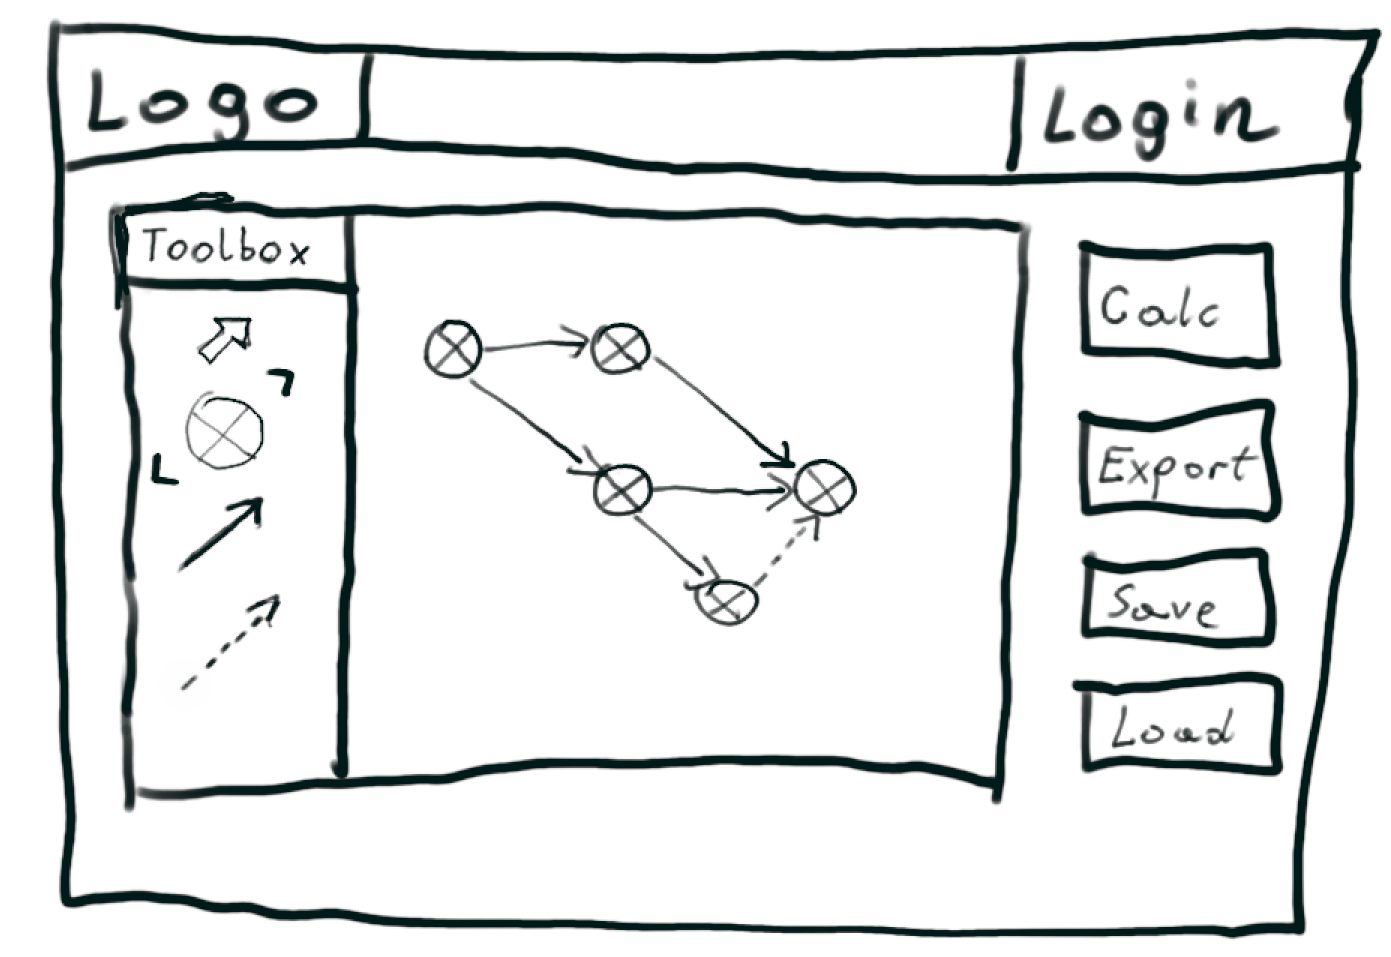
\includegraphics[width=0.9\linewidth]{main-window}
	\caption[Główne okno aplikacji]{Główne okno aplikacji}
	\label{fig:main-window}
\end{figure}

\section{Wymagania}
Wymagania projektowe zostaną zebrane w formie mapy historyjek użytkownika.

Kluczowe funkcjonalności aplikacji to
\begin{itemize}
	\item obsługa widoku strony www
	\item tworzenie diagramów
	\item analiza diagramów (np. dokonywanie obliczeń w celu wyznaczenia ścieżki krytycznej)
	\item generacja dodatkowych widoków (np. diagram Gantta)
	\item import i eksport diagramów
	\item obsługa sesji użytkownika (uwierzytelnianie, autoryzacja, zapisywanie diagramów na serwerze)
\end{itemize}
	
Każda z historyjek użytkownika powinna być związana z jedną z tych funkcjonalności. 

Każda z historyjek ma przypisanego aktora. Zidentyfikowano następujące role:
\begin{itemize}
	\item programista - przygotowuje aplikację
	\item autor - buduje diagram
	\item odbiorca - przegląda diagram
	\item użytkownik = autor+odbiorca
	\item właściciel aplikacji - posiada aplikację (może np zechcieć wyświetlać reklamy w celach zarobkowych, czy zbierać dane statystyczne) 
\end{itemize}

\subsection{Historyjki użytkownika tworzące ,,chodzący szkielet''}
Jest to minimalna funkcjonalność aplikacji wymagana, żeby uznać ją za użyteczną
\begin{itemize}
	\item jako programista chcę mieć zdefiniowany stos technologiczny, żebym wiedział w czym działać
	\item jako użytkownik chcę mieć dostępny widok strony podzielony na logiczne sekcje, żebym mógł korzystać ze wszystkich funkcjonalności
	\item jako programista chcę wiedzieć jak wygląda wysokopoziomowa architektura, żebym wiedział w jaki sposób zbudować system
	\item jako autor chce mieć dostępny toolbox żebym mógł wybrać jaką akcję chcę wykonać
	\item jako autor chcę rozpoczynać pracę od pustego obszaru roboczego jedynie z początkowym milestonem
	\item jako autor chcę móc dodać milestone do obszaru roboczego żebym mógł zacząć tworzyć plan projektu
	\item jako autor chcę móc połączyć dwa milestone'y linią reprezentującą wymaganą pracę, żebym mógł określić zależności czasowe
	\item jako autor chcę mieć możliwość przesuwania milestone'ów, żebym mógł przearanżować wygląd diagramu
	\item jako autor chcę móc dodać opis milestone'a, żebym wiedział czego on dotyczy
	\item jako autor chcę móc edytować nazwę milestone'a żebym mógł poprawić źle wprowadzoną nazwę
	\item jako autor chcę móc dodać złożoność czasową danego zadania, żebym mógł obliczyć kiedy kolejny milestone może zostać osiągnięty
	\item jako autor chcę móc edytować złożoność czasową, żeby dostosować plan do aktualnej sytuacji
	\item jako autor chcę móc dodać puste zależności, żebym mógł podkreślić zależności pomiędzy milestone'ami
	\item jako odbiorca chcę widzieć obliczone czasy osiągnięcia poszczególnych milestone'ów, żebym wiedział, czy plan projektu jest zgodny z celami biznesowymi
\end{itemize}
\section{Architektura}
Na podstawie opisu zidentyfikowano następujące klasy
\begin{itemize}
	\item User
	\item Toolbox
	\item Canva
	\item Model (diagram PERT)
	\item Milestone
	\item Link (połączenie pomiędzy dwoma milestone'ami)
	\item Task (zadania powiązane z danym linkiem)
	\item CriticalPath
	\item Gantt
\end{itemize}

Rysunek~\ref{fig:klasy} przedstawia wstępną propozycję diagramu klas. 
\begin{figure}[h]
	\centering
	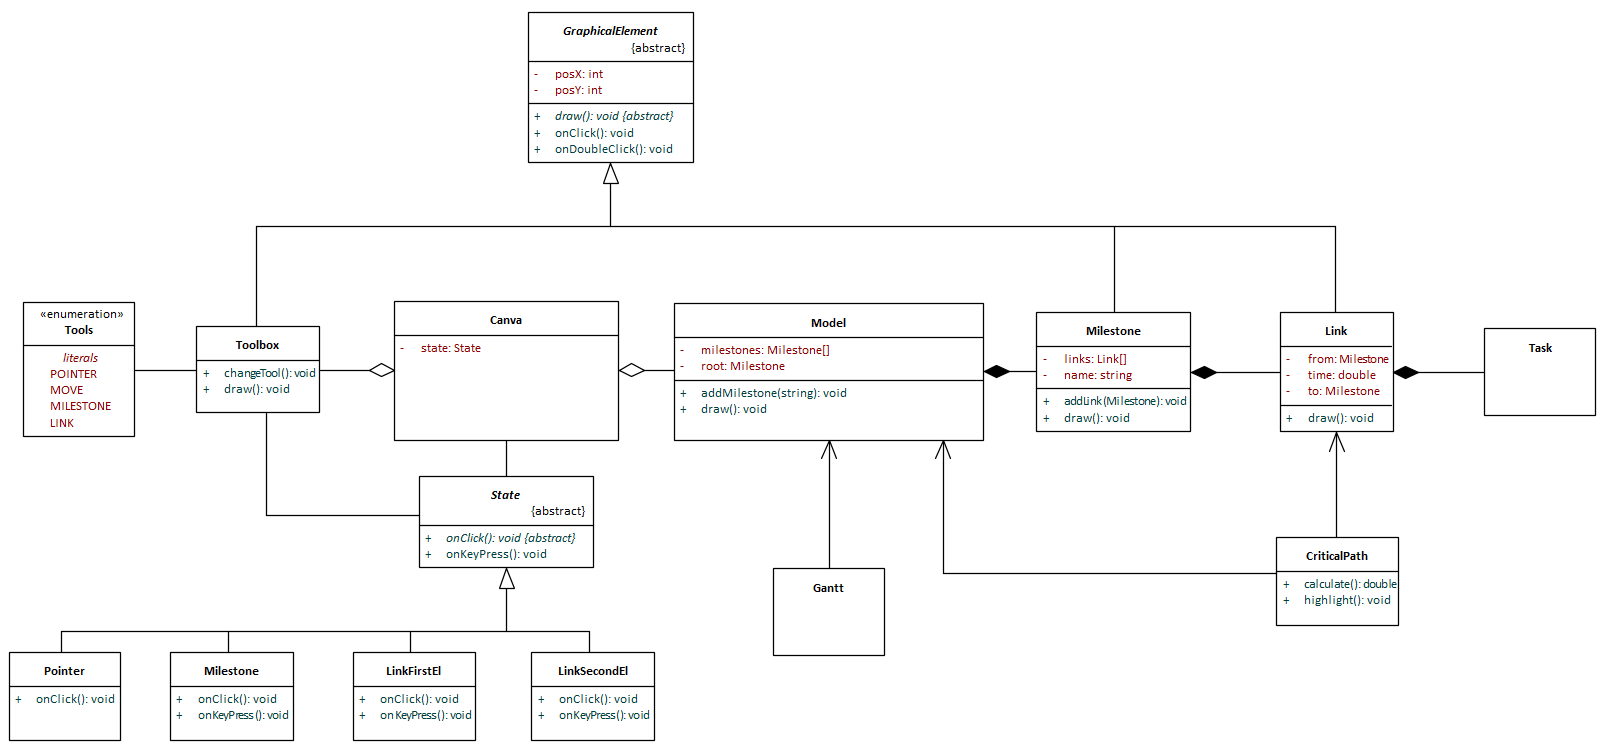
\includegraphics[width=1\linewidth]{img/klasy}
	\caption[Diagram klas]{Diagram klas (pierwsza iteracja)}
	\label{fig:klasy}
\end{figure}

Każdy z elementów, który można narysować rozszeraz klasę \textbf{GraphicalElement}

\subsection{Struktura danych}
Obiekt \textbf{Model} składa się z listy kamieni milowych (obiekty \textbf{Milestone}). Do tego zawiera on wskaźnik na element początkowy (wymagane jest to do obliczania ścieżki krytycznej).

Każdy milestone może być połączony z dowolną ilością innych kamieni milowych, dlatego zawiera on listę obiektów klay \textbf{Link}. Połączenia są skierowane od danego obiektu do innego.

Linki muszą być umieszczone zarówno w źródłowym, jak i docelowym milestone'ie, ponieważ przy przemieszczaniu dowolnego z nich, należy każdy link aktualizować

\subsection{Maszyna stanu}
\textbf{Toolbox} zawiera stan związany z wybranym narzędziem. Najbardziej skomplikowana (jak do tej pory) operacja to połączenie dwóch milestone'ów - musimy rozróżnić, czy wybrany został już pierwszy z nich, czy już wybrano docelowy. Również musimy sprawdzać, czy źródłowy i docelowy milestone to dwa różne obiekty.

Maszyna stanu została przedstawiona na Rysunku~\ref{fig:fsm-toolbox}

\begin{figure}
	\centering
	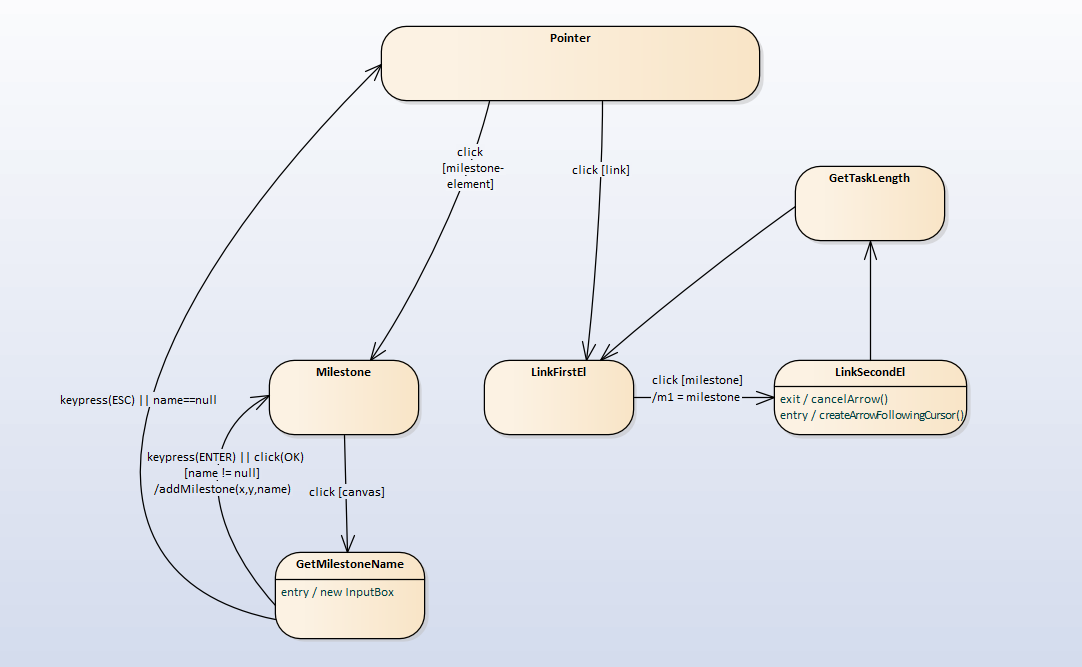
\includegraphics[width=1\linewidth]{img/fsm-toolbox}
	\caption[Maszyna stanu obiektu Toolbox]{Maszyna stanu obiektu Toolbox}
	\label{fig:fsm-toolbox}
\end{figure}
\section{Stos technologiczny}

Przy budowie aplikacji użyto następujących technologii

\subsection{Frontend}
\begin{itemize}
	\item HTML5
	\item CSS3
	\item JavaScipt
	\item Bootstrap - aspekty wizualne
	\item Konva.js - rysowanie w canvas
	\item jQuery - komunikacja z DOM, czy wsparcie AJAX
	\item Mocha.js, Chai.js, Sinon - testy jednostkowe oraz integracyjne
	\item Require.js - używanie wielu plikow js i eksport funkcji/klas pomiędzy nimi
\end{itemize}

\subsection{Połączenie}
Połączenie Frontendu z Backendem zrealizowano przy użyciu REST API.

Do testów REST API użyto \textbf{axios/superagent/request/...}

Zapytania wysyłane są przez frontend przy użyciu technologii AJAX.

\subsection{Backend}
\begin{itemize}
	\item Node.js
	\item Express
	\item TypeScript
	\item \textbf{coś do unit testów}
	\item MongoDB
\end{itemize}


\end{document}
